\documentclass[11pt,a4paper]{article}
\usepackage[utf8]{inputenc}
\usepackage[T1]{fontenc}
\usepackage{lmodern}
\usepackage[spanish,es-tabla]{babel}
\usepackage{amsmath,amssymb,mathtools}
\usepackage{booktabs,array,graphicx,float,xcolor,microtype,caption,enumitem,textcomp}
\newcommand{\euro}{\texteuro}
\usepackage[margin=2.5cm]{geometry}
\usepackage[hidelinks]{hyperref}
\captionsetup{font=small,labelfont=bf}
\newcommand{\E}{\mathbb{E}}
\newcommand{\Var}{\mathrm{Var}}
\newcommand{\VaR}{\mathrm{VaR}}
\newcommand{\TVaR}{\mathrm{TVaR}}
\title{\textbf{Tema 5 -- Preguntas de debate}\\[2pt]\large Teor\'ia de valores extremos y riesgos catastr\'oficos (POT / GPD)}
\author{Luiz Luzuriaga}
\date{M\'aster en Ciencias Actuariales y Financieras -- Universidad de Alcal\'a\\
Matem\'atica Actuarial de la Estabilidad y Solvencia de la Actividad Aseguradora\\ Curso 2026-27}
\begin{document}
\maketitle
\begin{abstract}\noindent
Las cuatro preguntas se responden con el Caso~1 (terremoto: $n=2.000$, $T=40$ a\~nos, $u=10$ M\euro, $N_u=80$, $\hat\xi=0{,}35$, $\hat\sigma=6$; $\VaR_{99,5}=28{,}35$, $\TVaR_{99,5}=47{,}46$ M\euro, $\lambda_u=2$) y el Caso~2 (inundaci\'on: $u=5$, $N_u=60$, $T=30$, $\hat\xi=0{,}25$, $\hat\sigma=4$), con simulaciones y bootstrap propios en Python y R.
\end{abstract}

\section*{Debate 1 -- Consecuencias de elegir el umbral demasiado bajo o demasiado alto}

\paragraph{Tesis.} El umbral decide el equilibrio entre sesgo y varianza, y su efecto se amplifica al pasar de la severidad por evento al capital anual: el VaR de severidad es robusto al umbral, pero el TVaR y el SCR no.

\paragraph{Umbral demasiado bajo.} Entran excesos que a\'un no est\'an en el r\'egimen asint\'otico de Balkema--Pickands--de Haan. La GPD intenta ajustar tambi\'en el cuerpo y, en general, \emph{subestima} $\xi$ (colas Burr, log-normal o con factores de variaci\'on lenta: la convergencia a $\xi$ es lenta) y desplaza $\hat\sigma$. En la tabla de la diapositiva ($\xi$ verdadero $0{,}33$) $u=5$ da $\hat\xi=0{,}21$ y un $\TVaR$ de $35{,}7$ frente al verdadero $42{,}7$ ($-16\%$); en la muestra de la pr\'actica de R, $u=5$ da $\hat\xi=0{,}25$ y $\TVaR=39{,}4$. Los intervalos son estrechos (muchos datos): \emph{falsa precisi\'on}. Consecuencia en capital: infracapitalizaci\'on de la cola.

\paragraph{Umbral demasiado alto.} Quedan pocos excesos ($N_u=23$ para $u=20$): $\hat\xi$ es muy inestable (de $0{,}06$ a $0{,}39$ entre $u=15$ y $20$ en la muestra de R) y los intervalos se abren (en la diapositiva, $\hat\xi=0{,}30$ con IC $[-0{,}22;0{,}82]$). Es posible que el \'optimo estad\'istico sea peor que el sesgo de un umbral bajo. Consecuencia: capital impredecible, con la posibilidad de $\hat\xi$ muy alto (capital desproporcionado) o negativo (cola acotada, pero sin base).

\paragraph{De la severidad al capital.}
\begin{center}
\small
\begin{tabular}{lrrr}
\toprule
 & $u$ bajo & $u=10$ & $u$ alto\\
\midrule
Diapositiva: $N_u$ & 520 & 139 & 24\\
$\hat\xi$ [IC 95\,\%] & 0,21 [0,11; 0,31] & 0,41 [0,18; 0,64] & 0,30 [$-$0,22; 0,82]\\
$\VaR_{99,5}$ (verdad 27,85) & 25,85 & 26,65 & 27,12\\
$\TVaR_{99,5}$ (verdad 42,67) & 35,68 & 44,14 & 40,31\\
\bottomrule
\end{tabular}
\end{center}
El VaR 99,5\,\% var\'ia $\approx5\%$ entre umbrales (est\'a cerca de los datos: unos 12 eventos lo superan); el TVaR, hasta un $24\%$ ($35{,}7$ a $44{,}1$), pues depende de $\hat\xi$. El efecto en el \emph{SCR anual} es mayor, porque el capital depende de la forma de la cola con frecuencia $\lambda_u=2$ (simulaci\'on, $\sigma=6$):
\begin{center}
\small
\begin{tabular}{rrrrrr}
\toprule
$\xi$ & 0,21 & 0,28 & 0,35 & 0,41 & 0,45\\
\midrule
SCR (M\euro) & 105,3 & 122,4 & 147,3 & 177,4 & 204,6\\
frente a $\xi=0{,}35$ & $-29\%$ & $-17\%$ & -- & $+20\%$ & $+39\%$\\
\bottomrule
\end{tabular}
\end{center}
Un error de $\pm0{,}07$ en $\hat\xi$ cambia el SCR en $-17\%/+20\%$.

\paragraph{C\'omo evitar ambos extremos.} (i) Gr\'afico del exceso medio y estabilidad de $\hat\xi$ y $\sigma^*=\hat\sigma-\hat\xi u$ con intervalos; elegir el \emph{menor} umbral a partir del cual ambos son compatibles con una constante. (ii) Sensibilidad documentada ($u=7{,}5$ y $12{,}5$ junto al elegido, como en la diapositiva). (iii) Umbrales por cuantiles (porcentaje de datos) y criterios autom\'aticos (Wadsworth, 2016; Scarrott y MacDonald, 2012). (iv) Reportar siempre IC del TVaR y del SCR. (v) Combinar con informaci\'on externa (modelos cat).

\paragraph{Nota de clase (5-nov).} Coincide con lo explicado en clase: con un umbral demasiado bajo se introducen importes m\'as peque\~nos, baja $\hat\xi$ y la cola se desplaza hacia abajo, de modo que la p\'erdida m\'axima a un a\~no se infravalora y el capital es menor; con un umbral demasiado alto el resultado puede sobreestimar o infraestimar, porque entra mucha volatilidad. Adem\'as, el cuantil 99,5\,\% de severidad es ``1 de cada 200 \emph{eventos}'', no ``1 en 200 \emph{a\~nos}'': con estos datos se supera cada 4 a\~nos, y si cambia la distribuci\'on cambia el dato.

\paragraph{Conclusi\'on.} Un umbral bajo infracapitaliza con una confianza injustificada; uno alto da un capital ruidoso. La decisi\'on debe documentarse con diagn\'osticos y sensibilidad, y el capital debe comunicarse con su intervalo.

\bigskip\hrule\bigskip

\section*{Debate 2 -- Si $N_u=80$ y $60$ proviniesen de solo 15 a\~nos}

\paragraph{Tesis.} El cambio no es solo estad\'istico: la frecuencia $\lambda_u=N_u/T$ se multiplica y la extrapolaci\'on a 200 a\~nos pasa de $5$ a $13$ veces el historial.

\paragraph{1. La frecuencia.} $\lambda_u=N_u/T$: con 80 excesos en 15 a\~nos, $\lambda_u=5{,}33$ eventos/a\~no (antes $2{,}0$); con 60 en 15 a\~nos, $4{,}0$ (antes $2{,}0$). La severidad condicionada a superar $u$ no cambia (misma GPD), pero cada a\~no ocurren $2{,}7$ veces m\'as eventos. El nivel de retorno $x_m=u+\frac\sigma\xi[(\lambda_um)^\xi-1]$ se desplaza:
\begin{center}
\small
\begin{tabular}{lrrr}
\toprule
 & $T=40$ ($\lambda_u=2$) & $T=15$ ($\lambda_u=5{,}33$) & Variaci\'on\\
\midrule
Caso 1: nivel 1-en-200 (M\euro) & 132,4 & 189,6 & $+43\%$\\
Caso 2: nivel 1-en-200 ($\lambda_u=4$) & 60,6 & 74,1 & $+22\%$\\
\bottomrule
\end{tabular}
\end{center}
El VaR 99,5\,\% de severidad por evento no cambia ($28{,}35$: depende de $n/N_u$, no de $T$), pero el periodo de retorno de ese VaR s\'i: $1/(\lambda_u\cdot P(X>x\mid X>u))$ pasa de $4$ a $1{,}5$ a\~nos. Es el ejemplo de que un VaR por evento no es un suceso 1-en-200.

\paragraph{2. La precisi\'on estad\'istica.} Si en 15 a\~nos el mismo proceso (con $\lambda_u=2$) solo produjese $N_u=30$ excesos, el error t\'ipico de $\hat\xi$ es $\approx(1+\xi)/\sqrt{N_u}$. Con un bootstrap param\'etrico (1.500 r\'eplicas, $\xi=0{,}35$, $\sigma=6$):
\begin{center}
\small
\begin{tabular}{lrr}
\toprule
 & $N_u=80$ (40 a\~nos) & $N_u=30$ (15 a\~nos)\\
\midrule
Desv. t\'ipica de $\hat\xi$ & 0,16 & 0,29\\
$\hat\xi$ IC 90\,\% & [0,05; 0,58] & [$-$0,22; 0,70]\\
$\VaR_{99,5}$ IC 90\,\% & [23,8; 33,1] & [21,6; 37,1]\\
Nivel 1-en-200 IC 90\,\% & [60; 272] & [39; 438]\\
Factor de extrapolaci\'on 200 a\~nos / historial & 5 & 13\\
\bottomrule
\end{tabular}
\end{center}
\begin{figure}[H]\centering
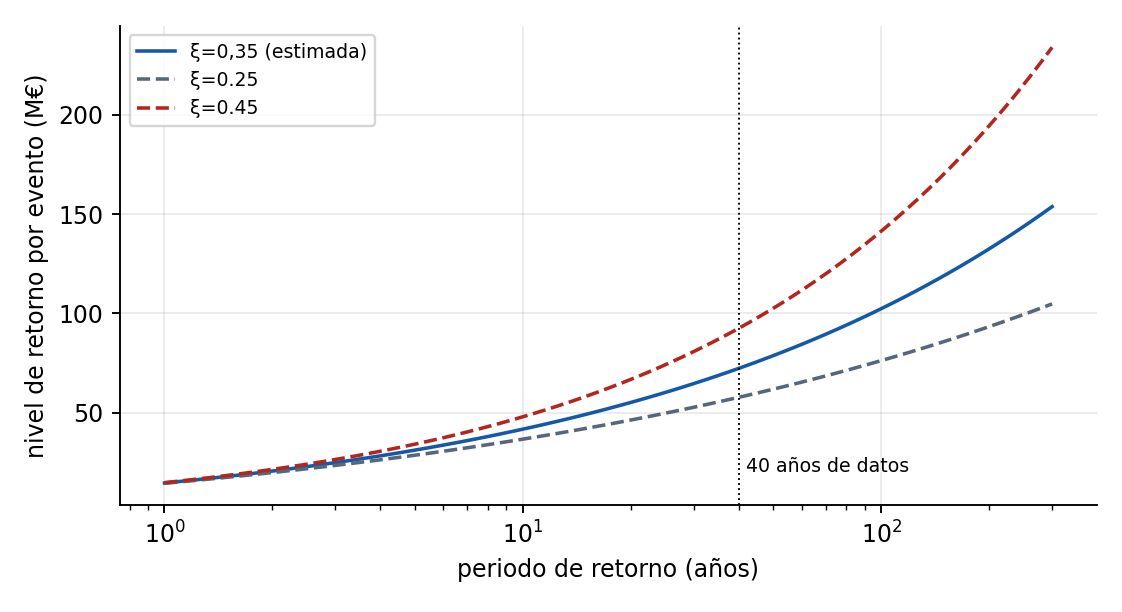
\includegraphics[width=.72\linewidth]{t5_f_debate2.png}
\caption{Niveles de retorno por evento en el Caso~1 para $\xi=0{,}25$, $0{,}35$ y $0{,}45$: la incertidumbre crece r\'apidamente m\'as all\'a de los datos.}
\end{figure}

\paragraph{3. Qu\'e confianza tendr\'ia.} Menor, y por tres razones: (i) intervalos m\'as anchos (el IC del nivel 200 a\~nos casi se duplica, con l\'imite inferior por debajo del actual m\'aximo observado); (ii) mayor factor de extrapolaci\'on ($>10$): por encima de unos 100 el resultado depende casi solo de $\hat\xi$, y la regla de prudencia exige comunicar IC y contrastar con informaci\'on externa; (iii) menor capacidad de diagnosticar estacionariedad, clusters y cambios de cobertura/inflaci\'on en una ventana corta (15 a\~nos no cubren un ciclo clim\'atico ni ver un evento tipo 1-en-50).

\paragraph{Nota de clase (5-nov).} Cuantos m\'as valores hay por encima del umbral, m\'as confianza en la inferencia, siempre que el comportamiento no var\'ie mucho (estacionariedad): con m\'as observaciones la estimaci\'on es m\'as coherente. Con $N_u=80$ y $60$ en 15 a\~nos hay los mismos excesos para estimar $\xi$, pero un historial m\'as corto: sube $\lambda_u$ y baja la confianza en la extrapolaci\'on a 200 a\~nos.

\paragraph{Qu\'e har\'ia.} Reforzar con datos externos (cat\'alogos hist\'oricos, datos sectoriales, modelos cat), usar priors informativos (enfoque bayesiano) o agrupar con carteras similares; fijar $\xi$ o restringirlo si hay justificaci\'on f\'isica; ampliar el margen de prudencia; y no extrapolar m\'as all\'a de unas decenas de veces el historial sin intervalos.

\bigskip\hrule\bigskip

\section*{Debate 3 -- Frecuencia creciente ($\approx25\%$ por d\'ecada) en el riesgo de inundaci\'on}

\paragraph{Tesis.} La tendencia debe entrar primero en la \textbf{frecuencia} $\lambda_u(t)$; la escala $\sigma$ y la forma $\xi$ solo si hay evidencia y base f\'isica; y separar exposici\'on de peligro.

\paragraph{1. Qu\'e depende del tiempo.}
\begin{itemize}[leftmargin=*,itemsep=2pt]
\item \textbf{$\lambda_u(t)$ -- s\'i, con prioridad.} Modelo $N_t\sim$ Poisson($\lambda(t)$), $\ln\lambda(t)=\beta_0+\beta_1(t-t_0)$. Con $25\%$ por d\'ecada, $\beta_1=\ln1{,}25/10=0{,}0223$. En una simulaci\'on de 40 a\~nos: $\hat\beta_1=0{,}025$ (EE $0{,}009$), $LR=7{,}47$, $p=0{,}006$.
\item \textbf{$\sigma(t)$ -- seg\'un covariables.} Si la intensidad del fen\'omeno (lluvia extrema, caudal) aumenta, los excesos son mayores: $\ln\sigma(t)=\gamma_0+\gamma_1 x(t)$ con covariables clim\'aticas (en \texttt{ismev::gpd.fit} con \texttt{ydat}, \texttt{sigl}).
\item \textbf{$\xi$ -- normalmente constante.} Es muy dif\'icil de estimar ($SE\approx(1+\xi)/\sqrt{N_u}$) y la convergencia es lenta; hacerlo depender del tiempo con 40 a\~nos suele sobreajustar. Se prueba en an\'alisis de sensibilidad.
\item \textbf{Separar exposici\'on y peligro.} Valores asegurados crecientes (más viviendas en zona inundable) son un cambio de exposici\'on y se tratan con \emph{as-if}/\emph{on-level} (reescalado de las p\'erdidas hist\'oricas a la cartera actual); lo que queda es cambio de peligro (clim\'atico). Confundirlos puede contar dos veces la tendencia.
\end{itemize}

\paragraph{2. Efecto en el SCR.} Con el Caso~2 ($u=5$, $\xi=0{,}25$, $\sigma=4$): el $\lambda_u$ estacionario ser\'ia $2{,}25$ (promedio de 40 a\~nos); con tendencia, el de 2025 es $3{,}62$ ($38\%$ m\'as). Resultados (simulaci\'on de $6\cdot10^5$ a\~nos):
\begin{center}
\small
\begin{tabular}{lrrr}
\toprule
 & Estacionario & Con tendencia (2025) & Variaci\'on\\
\midrule
$\lambda_u$ & 2,25 & 3,62 & $+61\%$\\
$E(S)$ anual (M\euro) & 23,2 & 37,4 & $+61\%$\\
SCR $=\VaR_{99,5}-E(S)$ & 74,4 & 90,2 & $+21\%$\\
Nivel de retorno 100 a\~nos (por evento) & 51,0 & 58,8 & $+15\%$\\
Nivel de retorno 200 a\~nos (por evento) & 62,7 & 72,0 & $+15\%$\\
\bottomrule
\end{tabular}
\end{center}
Suponer estacionariedad infravalora $\lambda_u$ actual y el nivel 1-en-100 en un $13\%$ ($51{,}0$ frente a $58{,}8$), y el SCR en un $17\%$ del valor correcto (74,4 frente a 90,2).

\paragraph{3. Horizonte.} Solvencia~II mira a un a\~no: se usa $\lambda_u(2026)$ extrapolado y no el promedio hist\'orico; para el reaseguro a varios a\~nos y para IFRS~17 (ajuste de riesgo sobre flujos futuros), la trayectoria de $\lambda_u(t)$ importa a\'un m\'as. Debe documentarse el supuesto de extrapolaci\'on (lineal en $\ln\lambda$), la sensibilidad (ventanas m\'oviles, tendencia reducida) y el riesgo de que la tendencia observada no persista.

\paragraph{Nota de clase (5-nov).} $\lambda_u$ es m\'as intuitivo y m\'as estable; $\xi$ puede ser estable dentro de un intervalo de umbrales, pero fuera de \'el da mucha variabilidad y puede hacer enorme la variabilidad de la distribuci\'on. Al estimar una tendencia se busca acertar m\'as, y eso se consigue modelando primero la frecuencia. Ejemplo de clase sobre calidad de la informaci\'on: una cartera de coches y otra de motos con la misma frecuencia pero severidad muy distinta; hay que estandarizar por exposici\'on, y tener en cuenta truncamientos y cambios de contrato o de ley (p.~ej. las reformas del baremo de tr\'afico, que cambiaron radicalmente las indemnizaciones; en M\'exico, la entrada de un baremo cambi\'o las cuant\'ias): el hist\'orico no refleja el riesgo actual.

\paragraph{Conclusi\'on.} Hacer depender del tiempo $\lambda_u$ (y, con covariables, $\sigma$), dejar $\xi$ constante, separar exposici\'on y peligro y calcular el SCR con la frecuencia vigente: el SCR estacionario infravalora en un quinto el requerimiento.

\bigskip\hrule\bigskip

\section*{Debate 4 -- Papel de la EVT en el dise\~no de un programa XL por capas}

\paragraph{Tesis.} La EVT aporta tres cosas: \emph{d\'onde} colocar las prioridades (periodos de retorno), \emph{cu\'anto} cuesta cada capa (prima pura con $\lambda_u$ y GPD) y \emph{cu\'anta incertidumbre} hay en cada precio, que crece con la altura de la capa.

\paragraph{F\'ormulas.} Con $u\le D$: $E[(X-D)^+\mid X>u]=\frac{\sigma+\xi(D-u)}{1-\xi}\big[1+\xi(D-u)/\sigma\big]^{-1/\xi}$; $EL_{L\,xs\,D}=\lambda_u\{E[(X-D)^+]-E[(X-D-L)^+]\}$; probabilidad anual de contacto $1-e^{-\lambda_uS(D)}$ y de agotamiento $1-e^{-\lambda_uS(D+L)}$; prima t\'ecnica $=EL+0{,}25\,\sigma_S$ y \emph{rate on line} $=$ prima$/L$.

\paragraph{Torre propuesta para el Caso~1} (M\euro; $\lambda_u=2$, $\sigma=6$; incertidumbre $\xi=0{,}35\pm0{,}10$):
\begin{center}
\small
\begin{tabular}{lrrrrrr}
\toprule
Capa & Per. retorno del punto de ataque & P(contacto) & $\xi=0{,}25$ & $\xi=0{,}35$ & $\xi=0{,}45$ & Prima t\'ecnica ($\pm$)\\
\midrule
10 xs 10 & 0,5 a\~nos & 86,5\,\% & 12,61 & 12,88 & 13,13 & $\pm2\%$\\
20 xs 20 & 1,9 a\~nos & 39--44\,\% & 6,15 & 7,21 & 8,22 & $-15/+14\%$\\
40 xs 40 & 9,0 a\~nos & 8--14\,\% & 2,50 & 3,77 & 5,17 & $-34/+37\%$\\
60 xs 80 & 52 a\~nos & 0,8--3,3\,\% & 0,93 & 1,82 & 2,97 & $-49/+63\%$\\
\bottomrule
\end{tabular}
\end{center}
(Las columnas $\xi$ son la prima t\'ecnica en M\euro; los rates on line, para $\xi=0{,}35$: $128{,}8\%$, $36{,}0\%$, $9{,}4\%$ y $3{,}0\%$.) La incertidumbre de $\xi$ pesa poco en las capas bajas y mucho en las altas: la capa m\'as alta (60 xs 80) var\'ia entre $0{,}93$ y $2{,}97$ M\euro.

\paragraph{Decisiones de dise\~no con EVT.}
\begin{enumerate}[leftmargin=*,itemsep=2pt]
\item \textbf{Prioridades por periodos de retorno.} El punto de ataque se fija con la frecuencia: retener los eventos que ocurren cada $\lesssim2$ a\~nos (la primera capa tiene $86{,}5\%$ de probabilidad de contacto y un rate on line superior al 100\,\%: es dinero que se recupera casi siempre, un canje de caja y no una transferencia de riesgo) y colocar capas sobre los de 2, 9 y 50 a\~nos.
\item \textbf{L\'imite de la torre.} Cubrir hasta el nivel 1-en-200 por evento ($132{,}4$): la torre 10 a 140 M\euro\ cubre el $1\!-\!1/200$ con una cola residual no asegurada que se mide con el TVaR o con la OEP.
\item \textbf{Precio y recargo.} La prima pura exige $\lambda_u$ y la GPD; el recargo remunera el capital del reasegurador y la incertidumbre de par\'ametros (principio de desviaci\'on est\'andar con $k=0{,}25$; con recargo proporcional del $30\%$, la capa 40 xs 20 cuesta $8{,}32$ M\euro\ frente a $9{,}48$). Para comparar ofertas hay que ver si el precio de las capas altas est\'a por encima de lo que implica el intervalo de $\xi$.
\item \textbf{Valor para el capital.} Cada capa reduce el SCR neto; el an\'alisis \emph{coste-beneficio} compara el ahorro de capital (coste de capital $\approx6\%$) con el recargo.
\item \textbf{Riesgo de base y dependencia.} Cl\'ausula horaria por evento, reinstalaciones (limitadas), y correlaci\'on entre peligros (inundaci\'on y terremoto), que condicionan el valor de una capa agregada.
\item \textbf{Validaci\'on y documentaci\'on.} Umbral y su sensibilidad, bondad de ajuste, IC y factor de extrapolaci\'on; contraste con modelos cat; y \emph{stress tests} de ``si $\xi$ fuese $+0{,}10$''.
\end{enumerate}

\paragraph{Nota de clase (5-nov).} Lo esencial es dividir bien cada una de las capas del reaseguro y apoyar la decisi\'on en estad\'istica (frecuencia, GPD, intervalos), porque con ello se ``juega'' con el reaseguro: se elige qu\'e retener y qu\'e ceder en cada tramo.

\paragraph{Conclusi\'on.} La EVT convierte la cola en precios y en un dise\~no explícito: prioridades por frecuencia, l\'imite por nivel de retorno y sensibilidad al par\'ametro de cola. Las capas altas dependen casi solo de $\hat\xi$ y por eso deben tarificarse con intervalo y con prudencia.

\subsection*{Referencias}
\begin{itemize}[leftmargin=*,itemsep=0pt]
\item Embrechts, P., Kl\"uppelberg, C. y Mikosch, T. (1997). \emph{Modelling Extremal Events for Insurance and Finance}. Springer.
\item Albrecher, H., Beirlant, J. y Teugels, J. L. (2017). \emph{Reinsurance: Actuarial and Statistical Aspects}. Wiley.
\item Scarrott, C. y MacDonald, A. (2012). A review of extreme value threshold estimation and uncertainty quantification. \emph{REVSTAT}, 10(1).
\item Wadsworth, J. L. (2016). Exploiting structure of maximum likelihood estimators for extreme value threshold selection. \emph{Technometrics}, 58(1).
\item McNeil, A. J. (1997). Estimating the tails of loss severity distributions using extreme value theory. \emph{ASTIN Bulletin}, 27(1).
\item Directiva 2009/138/CE (Solvencia~II), arts.~101 y 120--126.
\end{itemize}
\end{document}
